\documentclass{standalone}
% preamble: usepackage, etc.
\begin{document}
\chapter{BIB参考文献数据及软件使用}

(注意段落标题之间不能有空白必须有正文)(注意段落标题之间不能有空白必须有正文)(注意段落标题之间不能有空白必须有正文)(注意段落标题之间不能有空白必须有正文)(注意段落标题之间不能有空白必须有正文)

\label{chap4}

\section{JabRef安装}
以下为JabRef安装的安装方式:

1)安装地址:\href{https://www.jabref.org/}{官网地址,点击跳转};

2)点击download,如图\ref{fig_3}所示;
\begin{figure}[htbp]
	\centering
	
\includegraphics[width = \textwidth]{a4.pdf}
	\bicaption{安装方式}{Installation mode}
	\label{fig_3}
\end{figure}

3)双击JabRe图标按提示进行安装,如图\ref{fig_4},安装完成后无需进行Java环境变量的配置;
\begin{figure}[htbp]
	\centering
	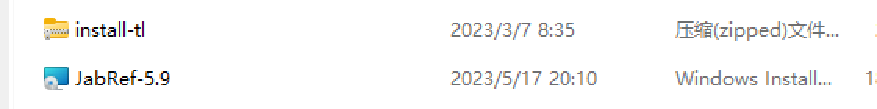
\includegraphics[width = \textwidth]{a5.pdf}
	\bicaption{直接安装}{Direct installation}
	\label{fig_4}
\end{figure}

4)设置中文模式:Options-> Preference-> General,设置语言为“中文简体”。


\section{使用方法}
以下为JabRef的使用方法:

1)文件——新建库——ctrl+s保存,选择一个文件夹放进去,进行命名,如图\ref{fig_5};
\begin{figure}[htbp]
	\centering
	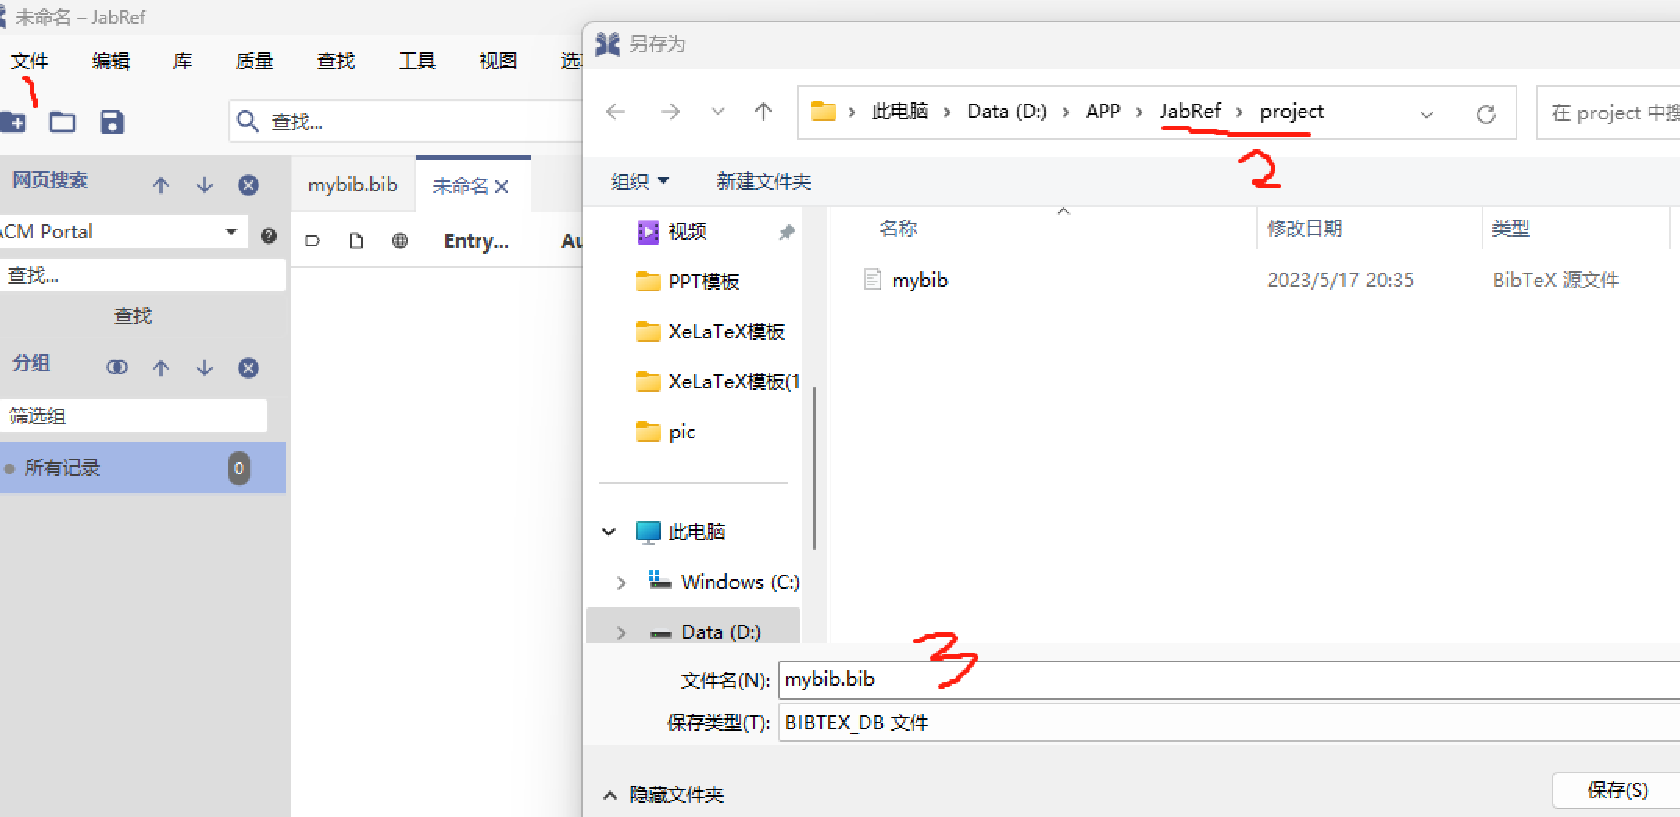
\includegraphics[width = \textwidth]{a6.pdf}
	\bicaption{保存文件}{Save file}
	\label{fig_5}
\end{figure}

2)添加参考文献:新建一个article,点击图标栏的这个加号,如图\ref{fig_7},
\begin{figure}[htbp]
	\centering
	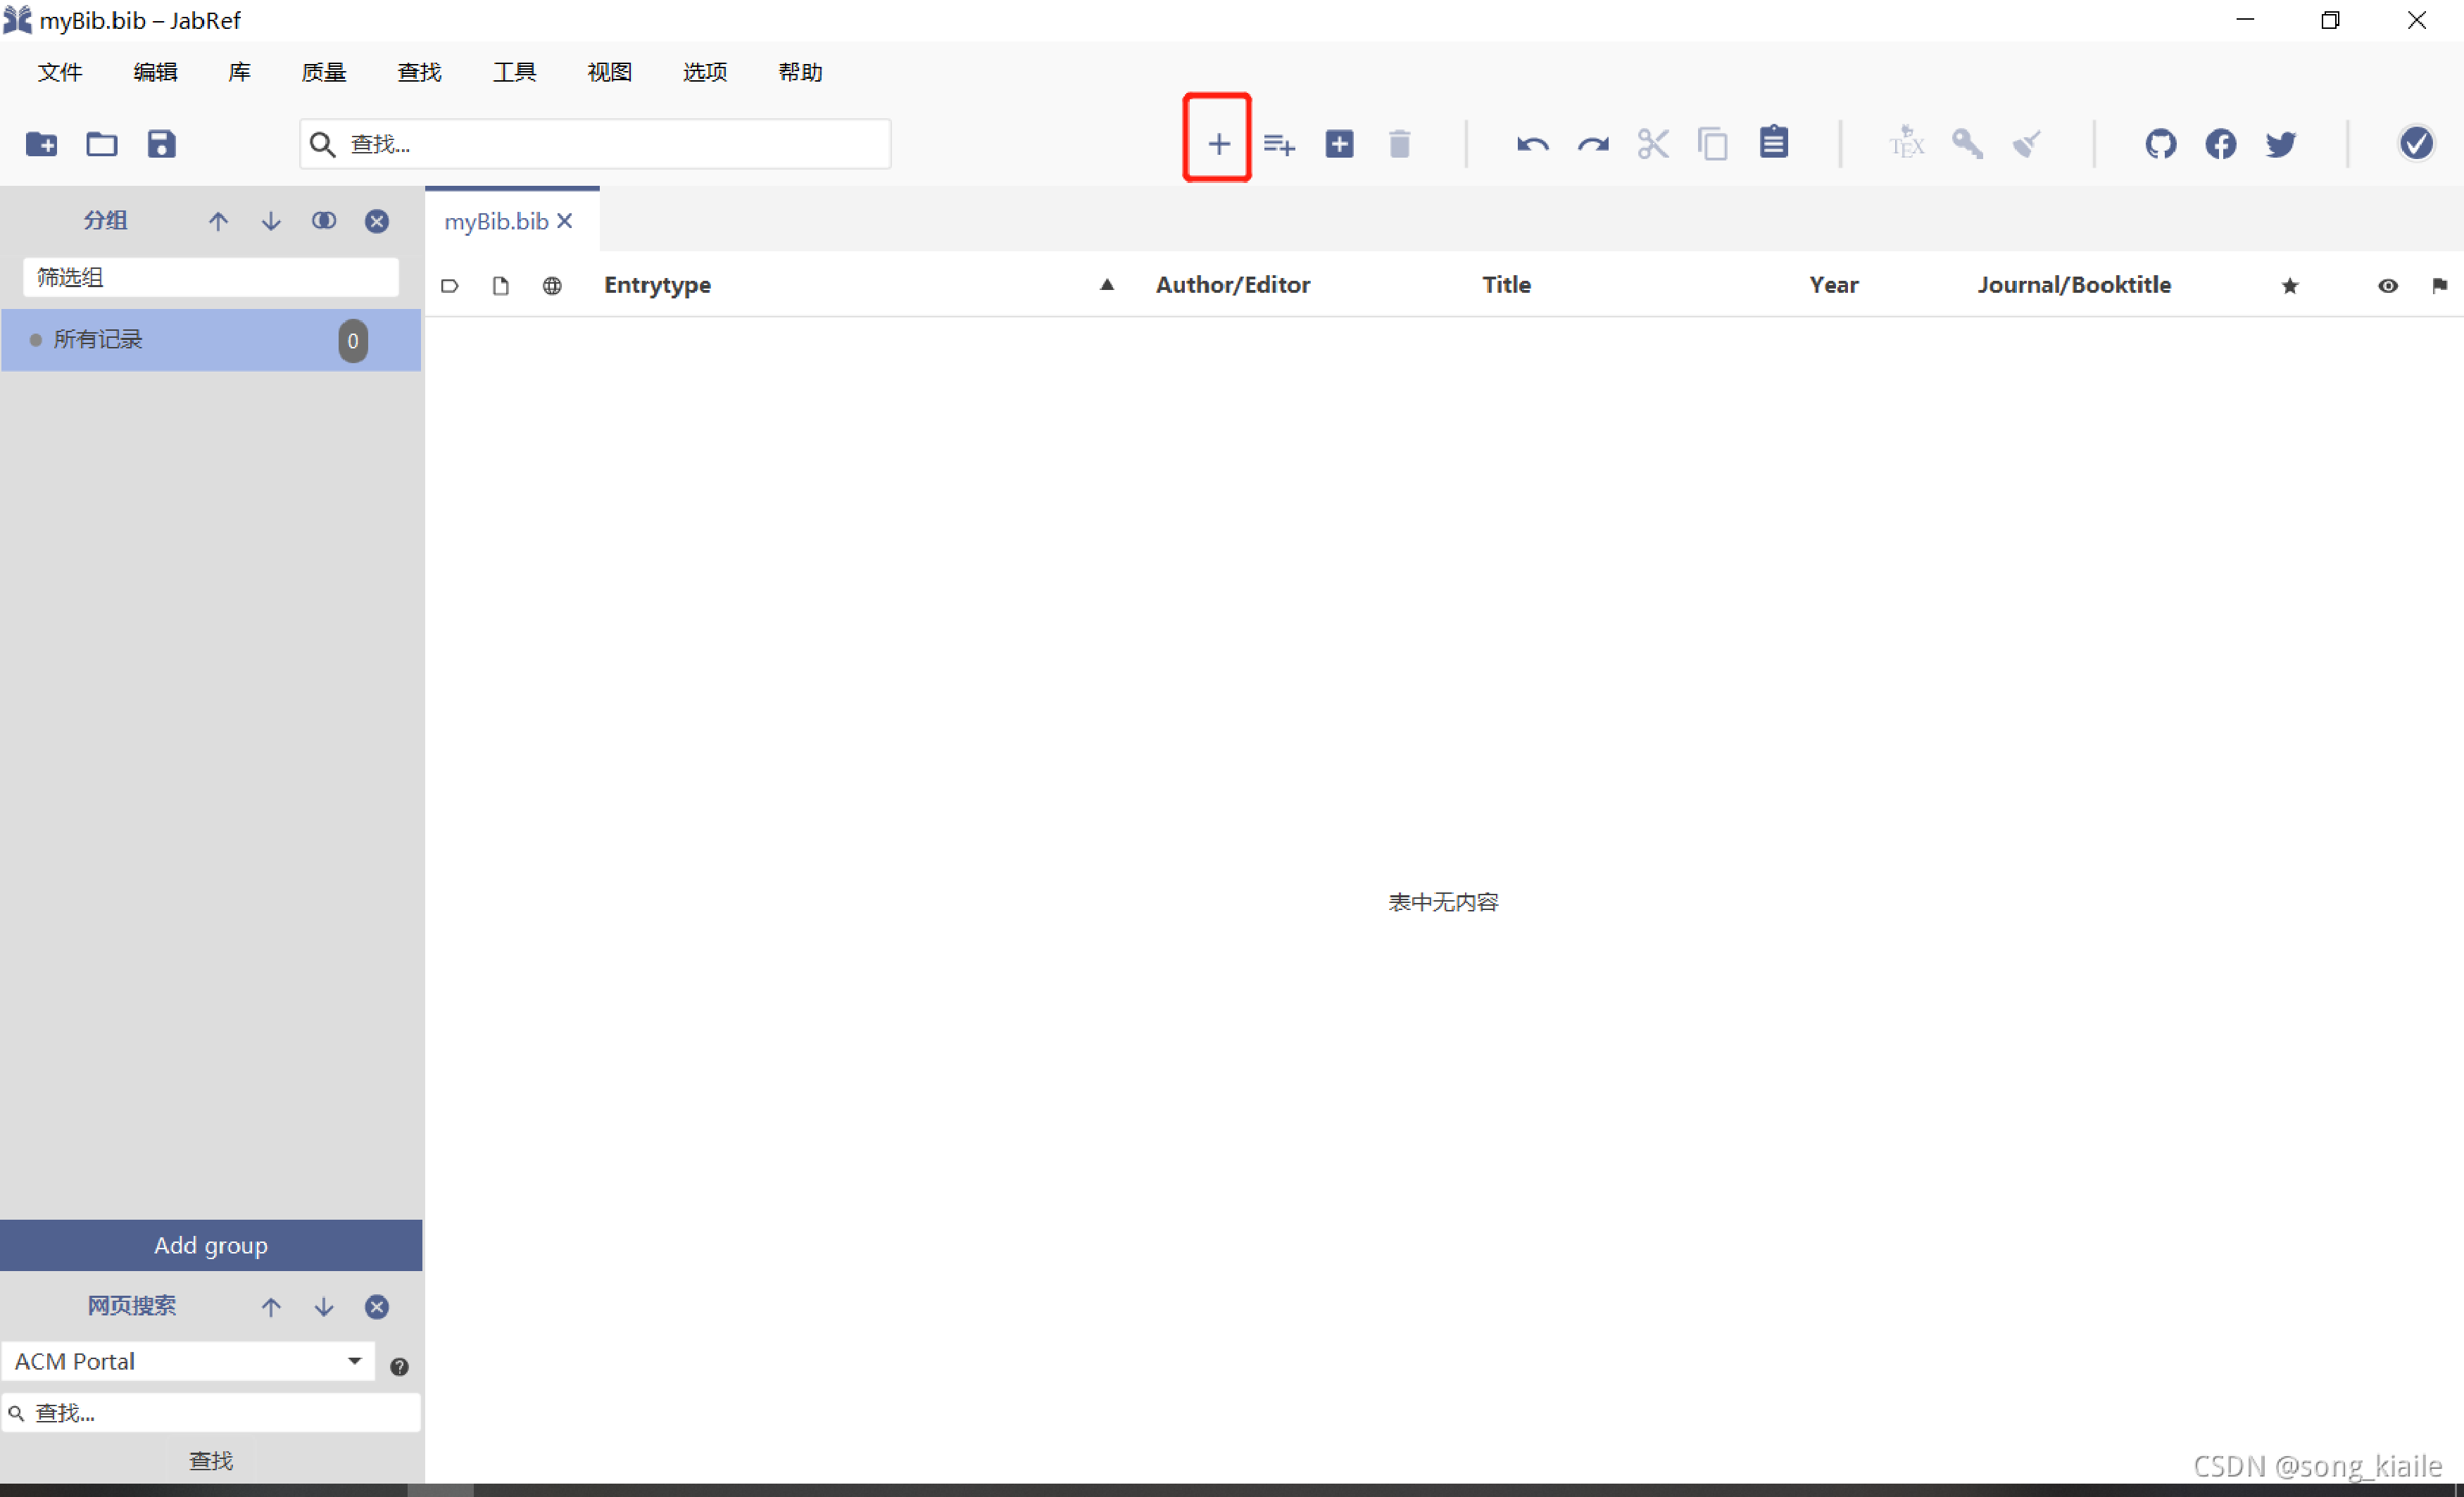
\includegraphics[width = \textwidth]{a8.pdf}
	\bicaption{新建文件}{New file}
	\label{fig_7}
\end{figure}
设置成功后如图\ref{fig_6}所示;
\begin{figure}[htbp]
	\centering
	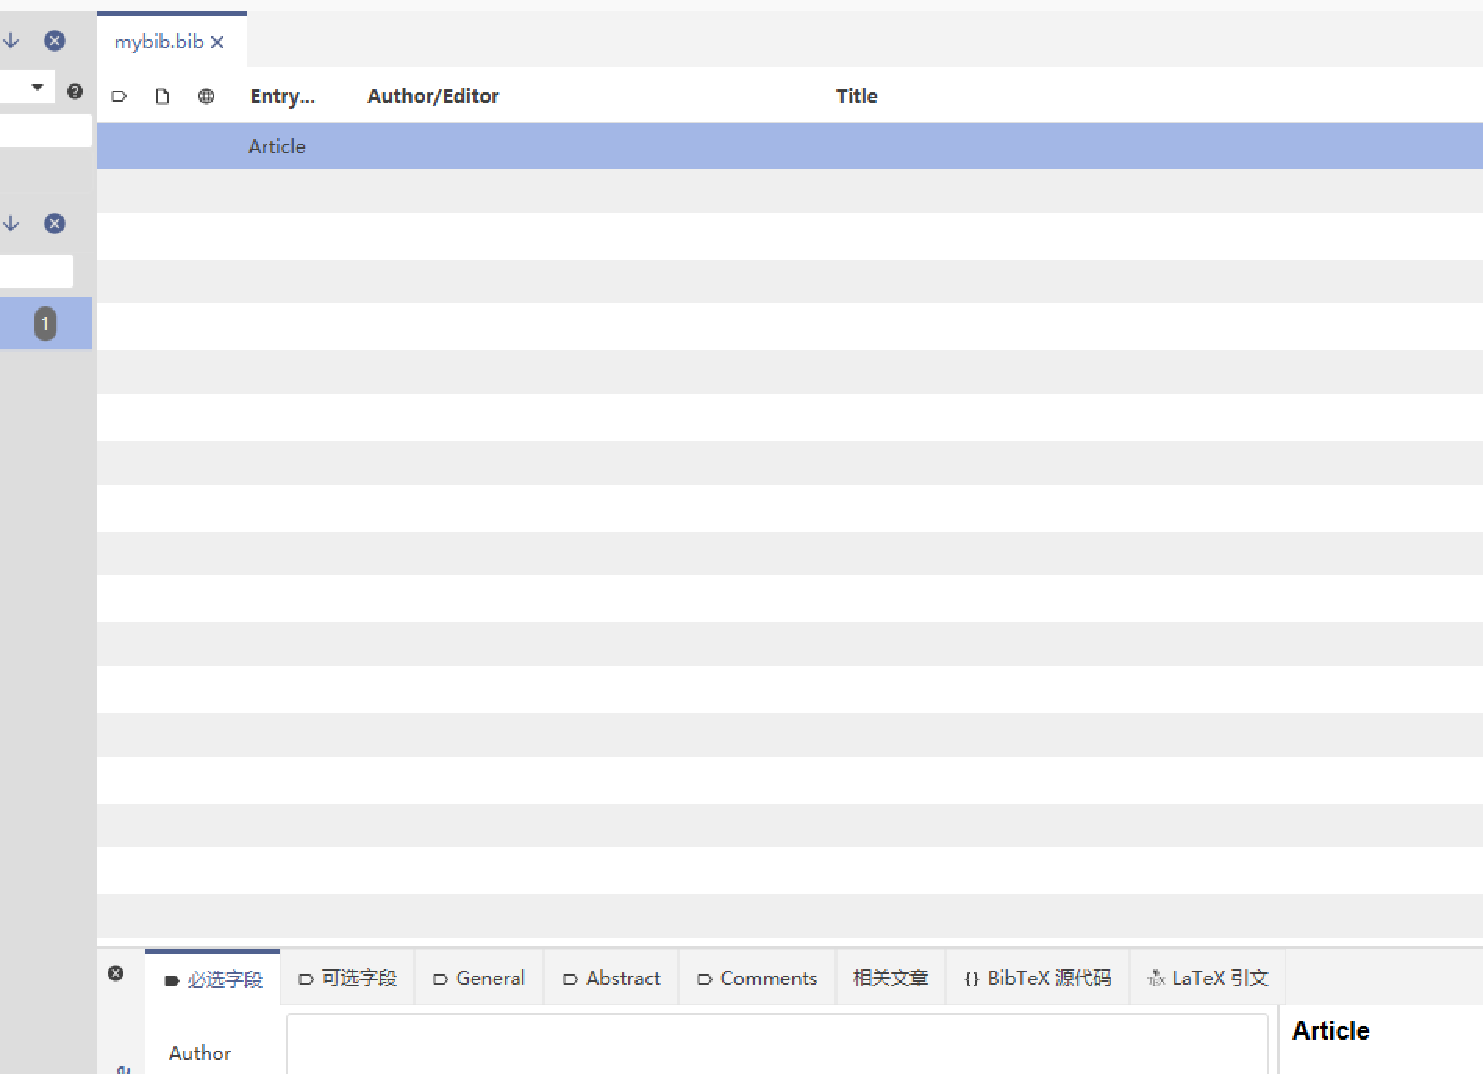
\includegraphics[width = \textwidth]{a7.pdf}
	\bicaption{新建成功界面}{Creating a successful screen}
	\label{fig_6}
\end{figure}

3)谷歌学术随便搜一个文献,复制BibTex,粘贴到下面这个区域,如图\ref{fig_8},然后保存就可以了;
\begin{figure}[htbp]
	\centering
	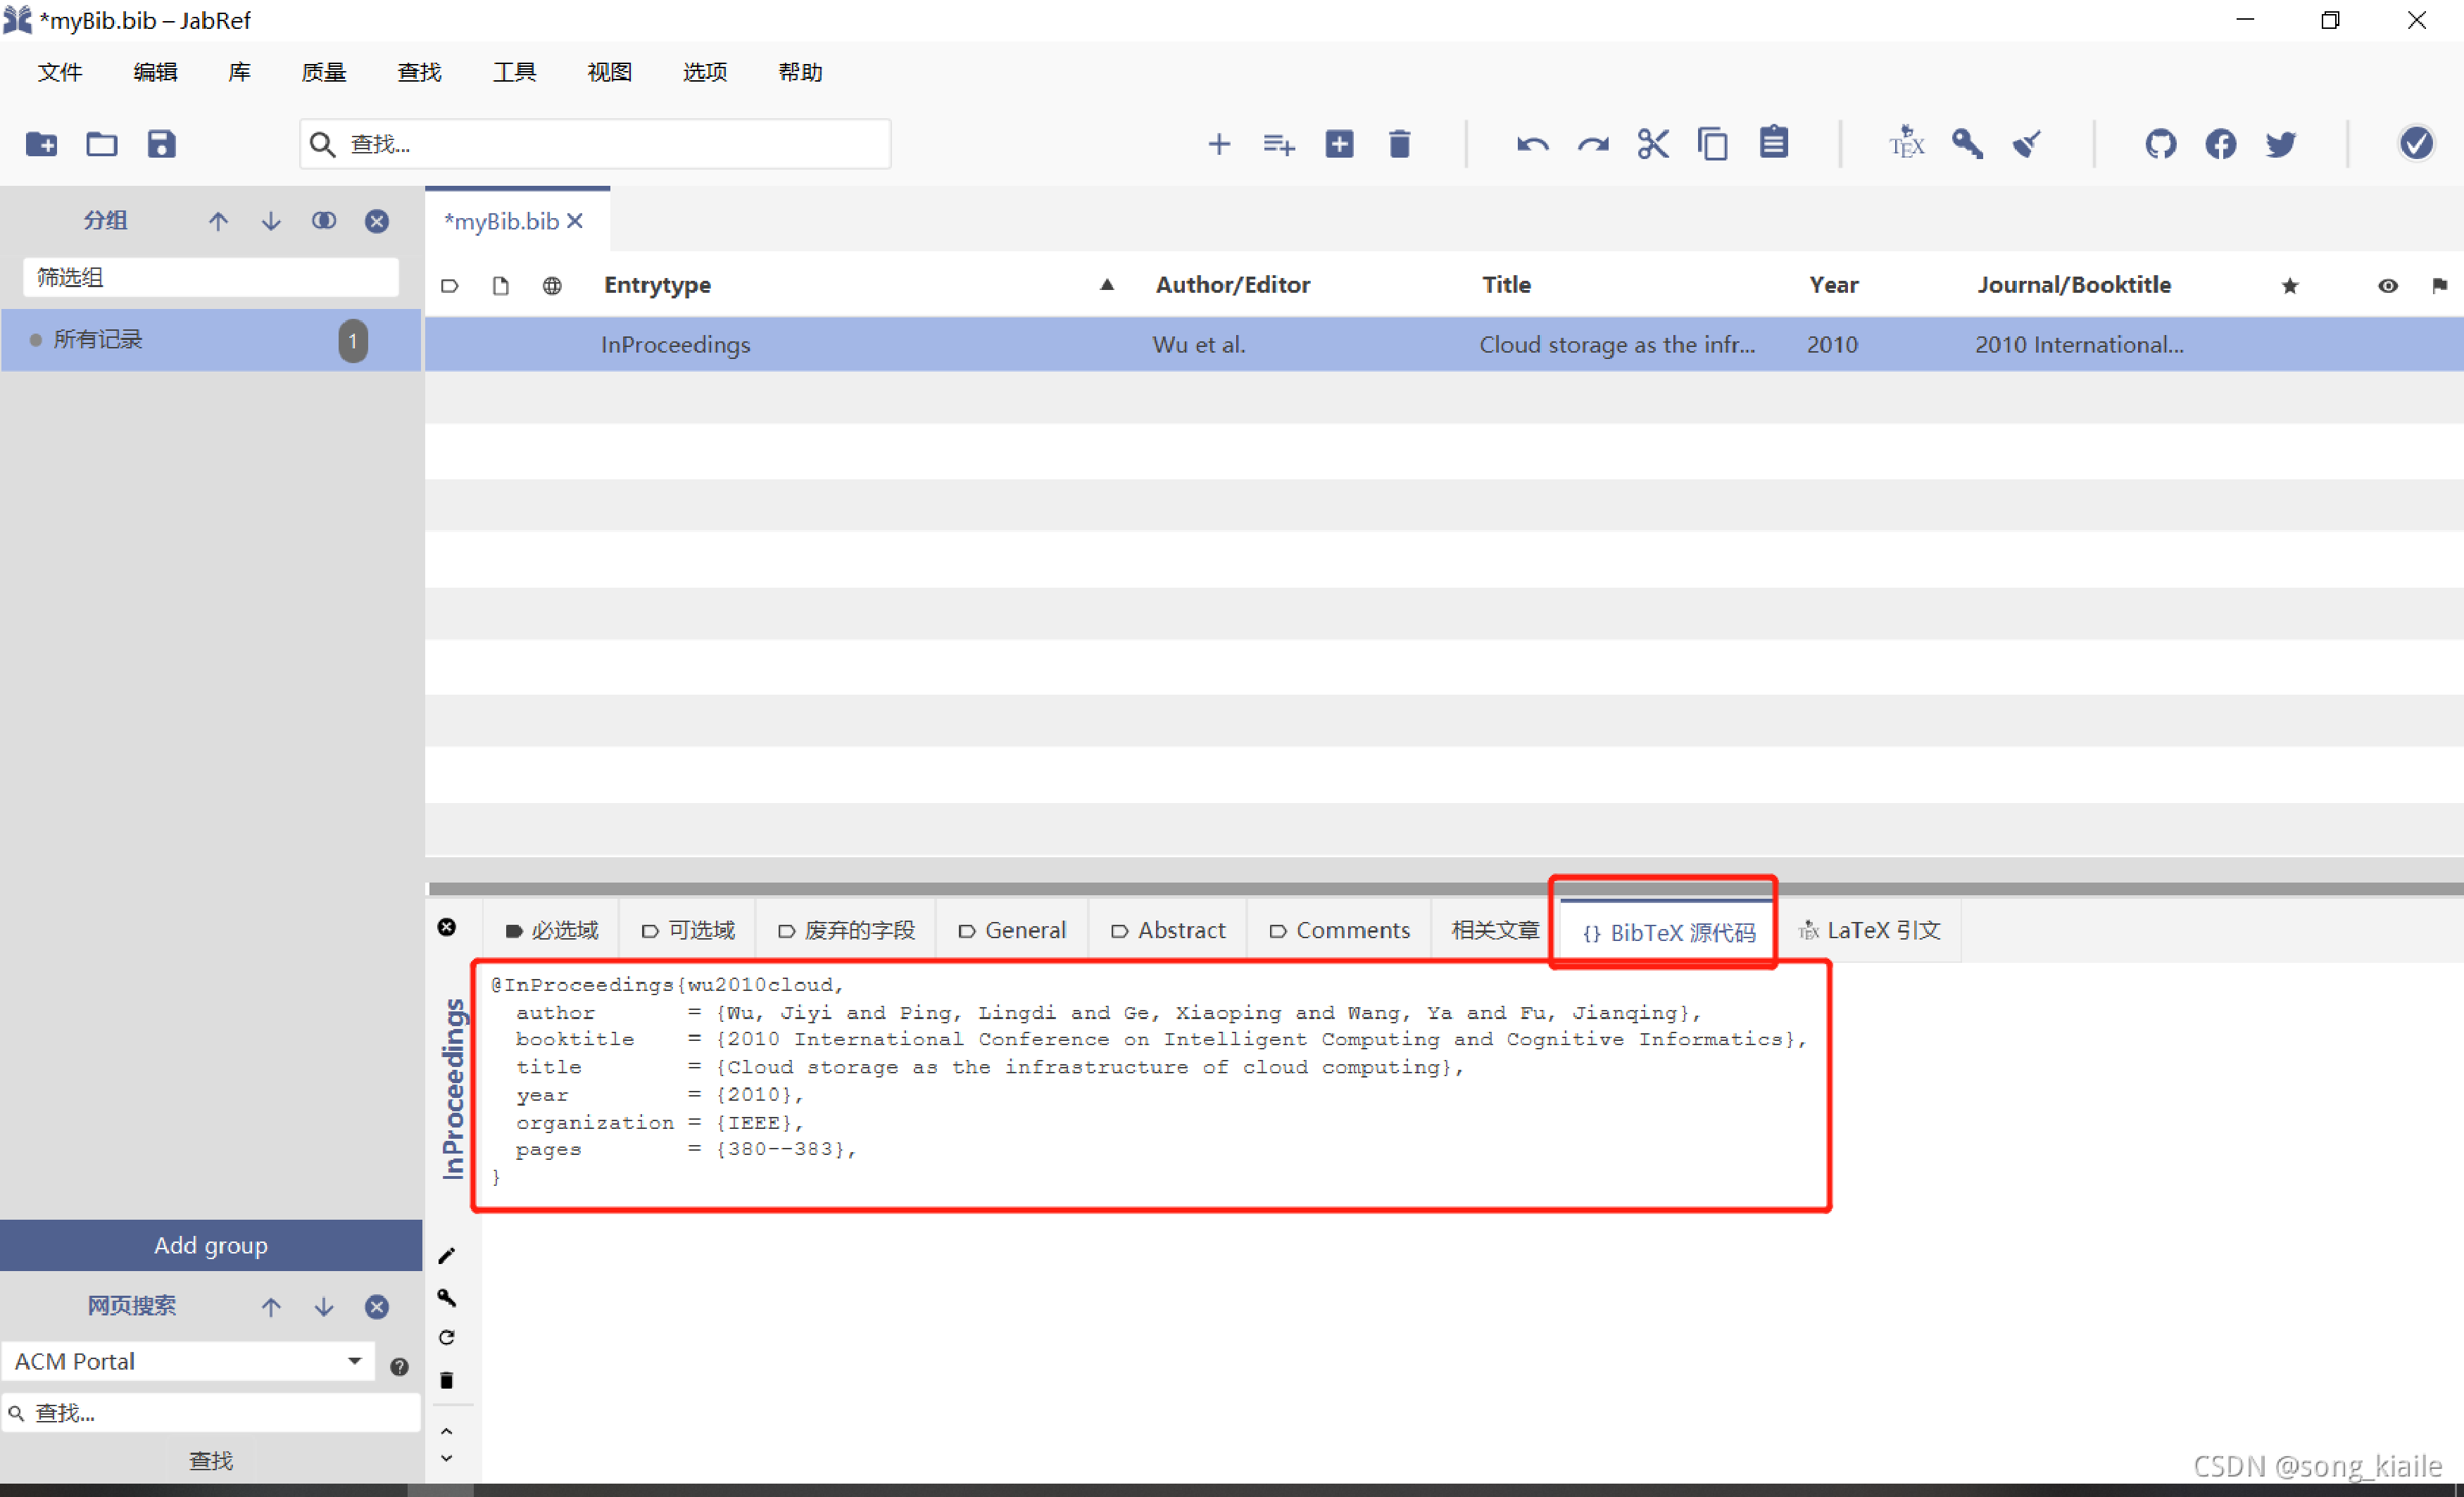
\includegraphics[width = \textwidth]{a9.pdf}
	\bicaption{参考文献界面}{Reference interface}
	\label{fig_8}
\end{figure}

4)可以看到“必选域”这里已经有了作者,标题,年份等信息,如图\ref{fig_9};
\begin{figure}[htbp]
	\centering
	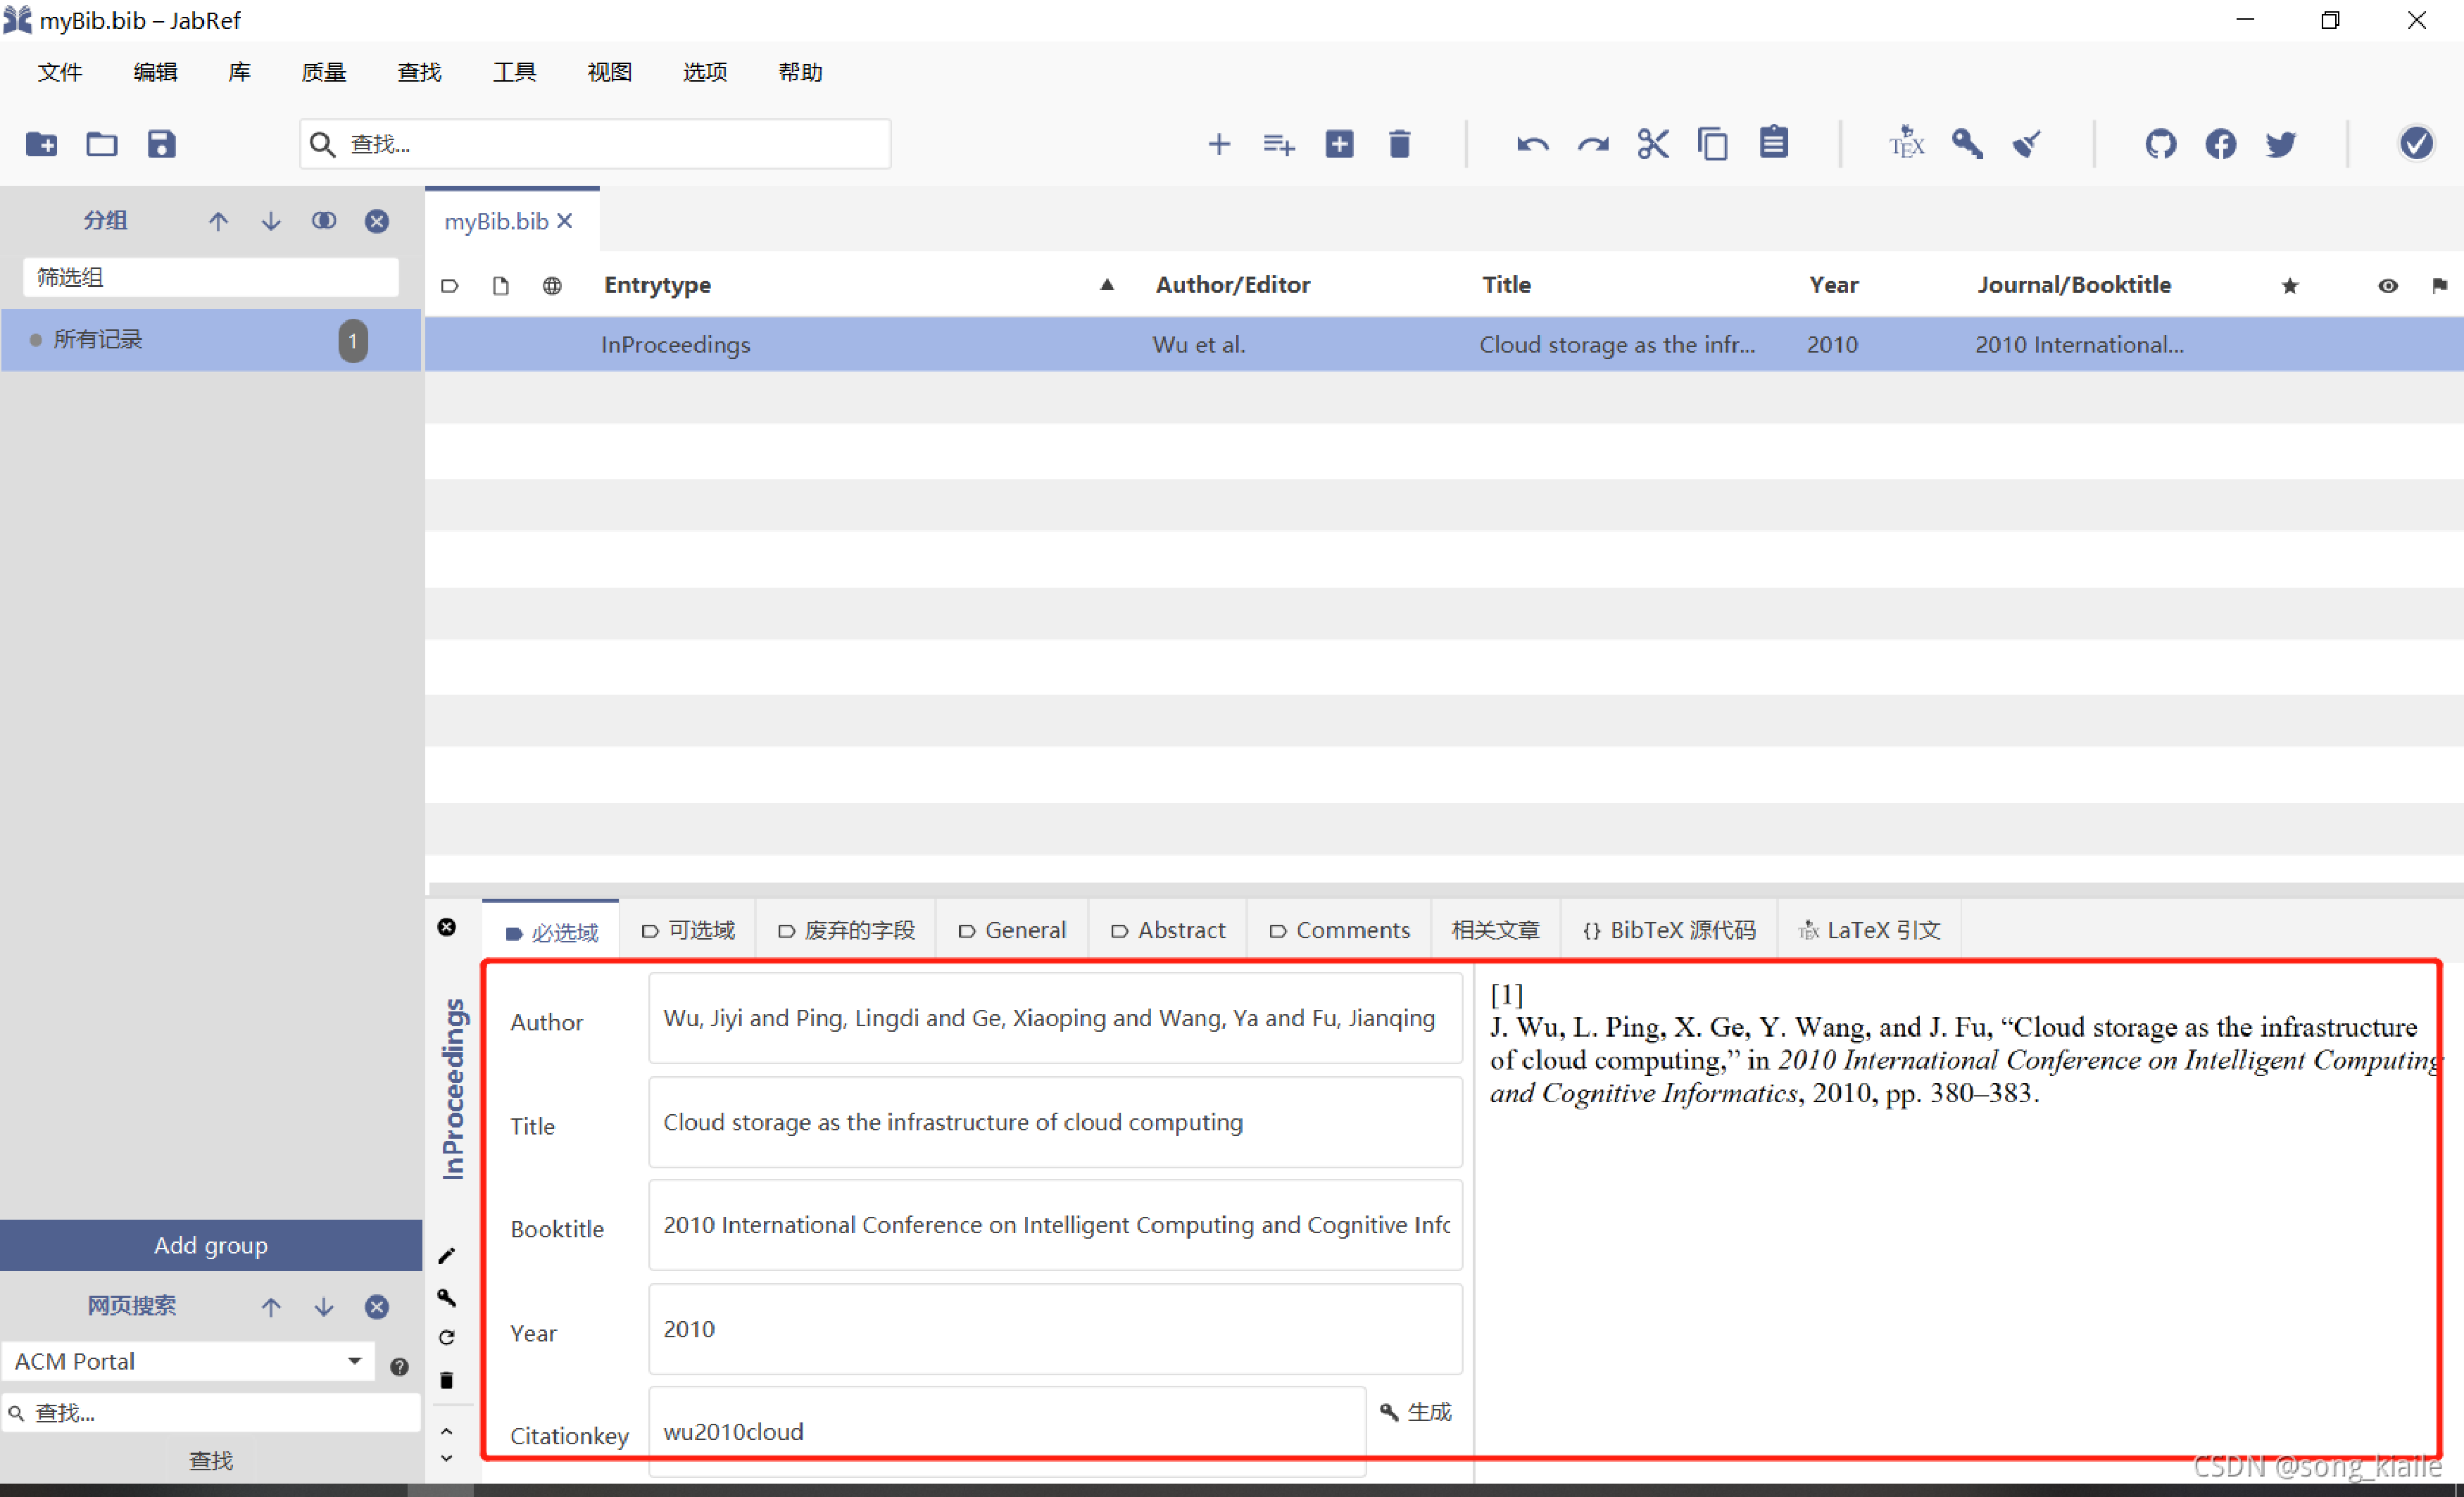
\includegraphics[width = \textwidth]{a10.pdf}
	\bicaption{参考文献}{Reference}
	\label{fig_9}
\end{figure}

5)最后将BibTex源代码粘贴到reference参考文献里面。


\section{文献引用}

1)添加文献:可以通过手动输入文献信息、导入文献文件或者通过DOI号码添加文献;

2)组织文献:可以通过添加关键词、标签、笔记等方式对文献进行分类和组织;

3)搜索文献:可以使用JabRef内置的搜索功能快速找到需要的文献,如图\ref{fig_10}所示;
	\begin{figure}[htbp]
		\centering
		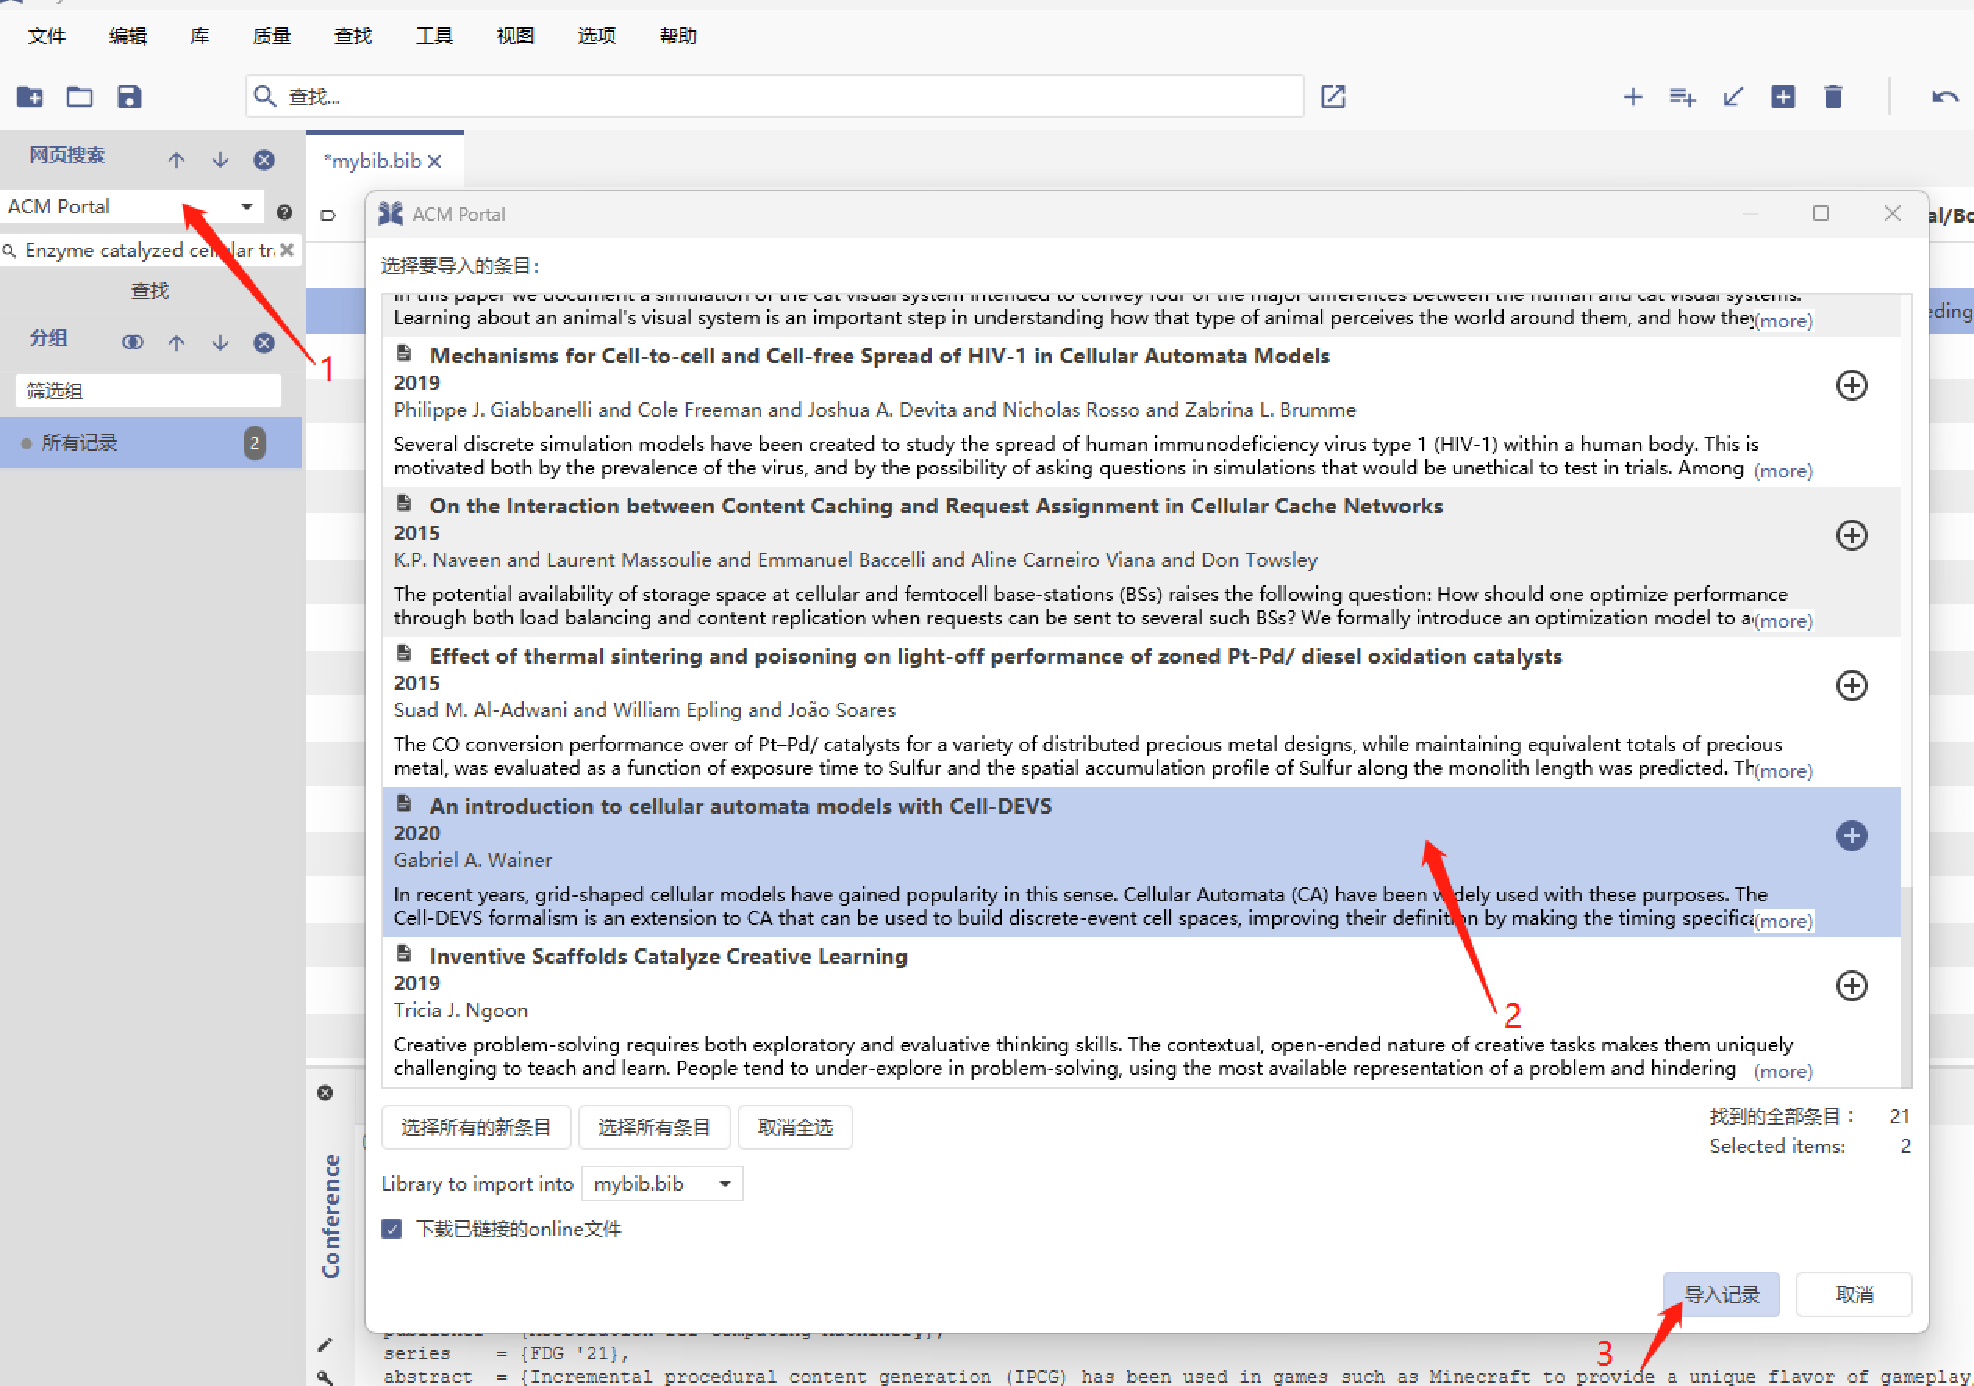
\includegraphics[width = \textwidth]{a13.pdf}
		\bicaption{搜索文献}{Search literature}
		\label{fig_10}
	\end{figure}
	
4)导出文献:可以将选定的文献导出为各种格式,如BibTeX、EndNote、RIS等;

5)连接文献库:可以将JabRef与外部文献数据库(如PubMed、Google Scholar等)连接,以便自动获取文献信息;

6)插入引用:可以在写作时轻松插入引用,并自动生成参考文献列表。

以上是JabRef基本使用教程的简要介绍,更多详细操作请参考JabRef的官方文档或其他相关资料。

\section{参考文献}

(注意段落标题之间不能有空白必须有正文)文献这里最好用google学术,把论文的卷、期和页面查准,如果不全,生成的也会缺失。

\subsection{参考文献引用方法}

上面的箭头为本文件reference粘贴过来的Bib参考文献,下面的箭头为引用方式,两者名称一致,如图\ref{fig_12}。每一次添加文献都需要按图\ref{fig_1}所示的编译方法编译,否则编译不成功,无法正确引用参考文献。
\begin{figure}[htbp]
	\centering
	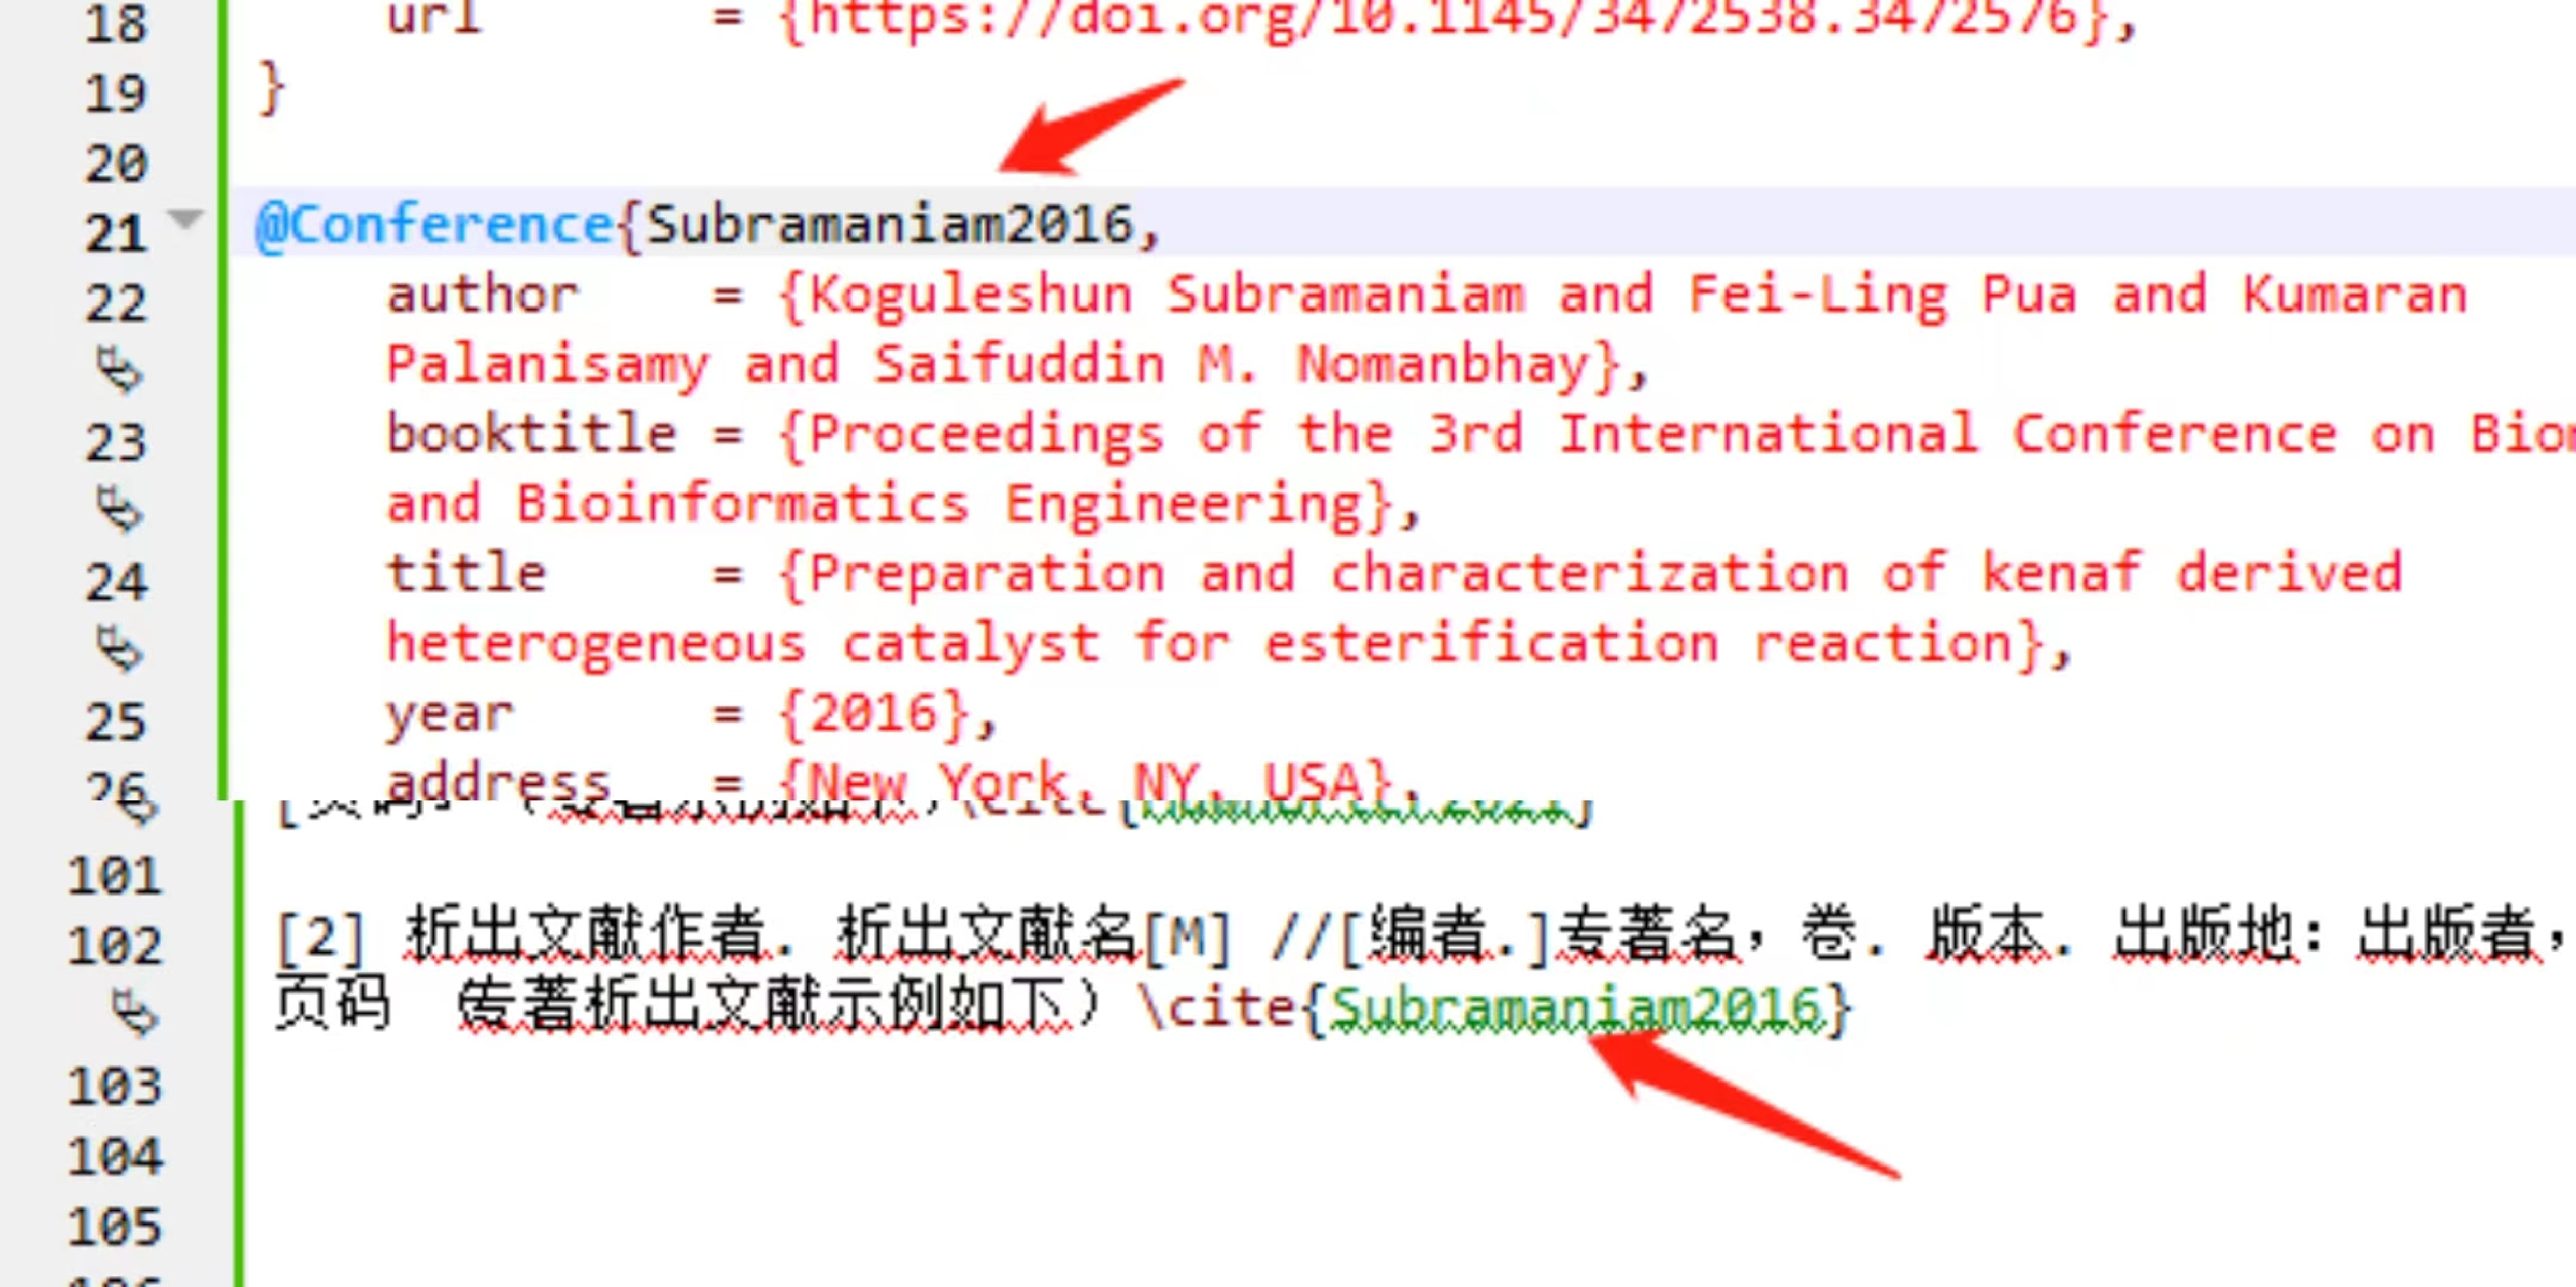
\includegraphics[width = \textwidth]{a14.pdf}
	\bicaption{引用方法}{Reference method}
	\label{fig_12}
\end{figure}

注:author如果有多个,中间用and连接,否则会出错。



\subsection{参考文献引用示例}
[1]	作者. 书名[M].  版本(第1版不注). 出版地:出版者,出版年: [页码](专著示例如下)\cite{Mawhorter2021}

[2]	析出文献作者. 析出文献名[M] //[编者.]专著名,卷. 版本. 出版地:出版者,出版年: 页码 (专著析出文献示例如下) \cite{Subramaniam2016}

[3]	原作者. 原文书名[M]. 出版地:出版者,出版年:页码(in Chinese) (译著示例如下) \cite{ref_1}

[4]	用户手册名[M]. 出版地:出版者,出版年 (用户手册示例如下) \cite{ref_2}

[5]	作者. 题名[J]. 期刊名,年,卷(期):页码//作者. 题名[N]. 报纸名,年-月-日(版次)(连续出版物示例如下) \cite{ref_3}

[6]	作者. 题名[J/OL].期刊名,年,卷(期):页码[引用日期]. 获取和访问路径其中引用日期用投稿日期替换即可。(连续出版物中的析出文件,以期刊为例示例如下) \cite{ref_4}

[7]	作者. 题名[C](后面无句号) //会议论文集名称。出版地:出版者,出版年:页码(若是英文文献,英文会议论文集的题目请以“Proceedings(此处有s) of …开始,每个单词全拼,每个实词首字母大写” 若是中文文献,直接写会议论文集的题目) \cite{ref_5}

[8]	作者. 题名[学位论文或技术报告][D或R].保存地:保存单位(指该论文被具体保存的地方,如北京大学图书馆,清华大学计算机科学与技术系),保存年(学位论文或技术报告示例如下) \cite{Anderson1998}

[9]	专利申请者. 专利题名:专利国别, 专利号[P]. 公告日期或公开日期[引用日期](专利文献示例如下) \cite{ref_6}

[10]	起草责任者.  标准代号 标准顺序号—发布年  标准名称[S]. 出版地:出版者,出版年(也可略去起草责任者、出版地、出版者和出版年,技术标准示例如下) \cite{ref_7}

注:misc标签引用时无法正常引用,改用online标签。

[11]	作者. 题名[OL]. [用投稿日期代替即可]. 获取和访问途径(电子文档示例如下) \cite{Baskaran2008}

\end{document}